% https://tex.stackexchange.com/a/468429
\documentclass{beamer}
\usepackage{tikz}
\usetikzlibrary{positioning}

\usetikzlibrary{overlay-beamer-styles}

\tikzset{block/.style={rectangle, draw, text width=6em, text centered, rounded corners, minimum height=3em}}

\begin{document}

    \begin{frame}

    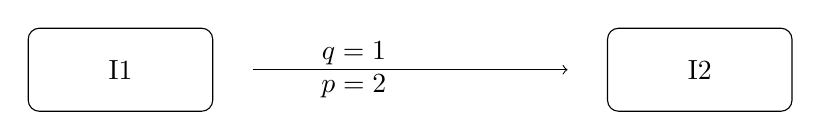
\begin{tikzpicture}
    \node [block] (I2) {I2};
    \node [block] [left=5cm of I2] (I1) {I1};

    \path[->,alt=<2>{red}{black}] (I1) edge[shorten >=0.5cm, shorten <= 0.5 cm] node [right, near start, align=center] {$q=1$\\$p=2$} (I2);

    \end{tikzpicture}

    \end{frame}
\end{document}
